In practice, arbitrage is the process of buying something at price $x$
and instantly selling it a price $y$ where $x<y$. Arbitrage is
risk-free, if we make some assumptions; since we perform it instantly
we can guarantee that $x<y$, and we do not take into account the
inherit vulnerabilities of bugs in smart contracts.

\subsection{LOB arbitrage}
When determining the arbitrage opportunity it is a bit more
complicated, since prices of assets are not static, but determined by
market behaviors. As we defined in the background section, there are
two main forms of exchanges, the simpler one being the limit order
book. When performing arbitrage on LOB DEXes, we check if there is some
asset (ABC) that has an overlapping price. An example of this can be
seen in figure \ref{fig:ArbLOB}, here we see that we can buy the ABC
asset at exchange Y and sell it at exchange X, and we can do that for
the overlapping limit orders.
\begin{figure}[h]
\centering
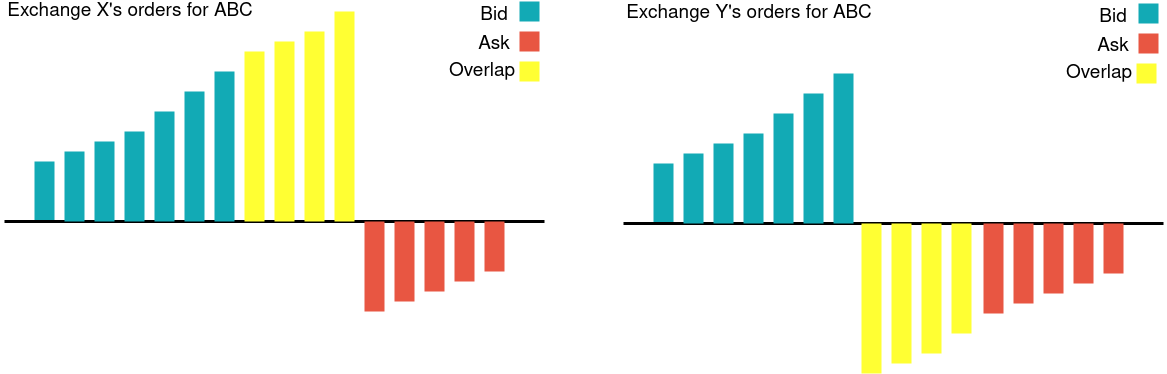
\includegraphics[width=0.7\textwidth]{assests/Flash-loans-Arbitrage-Overlap-1}
\caption{Arbitrage on LOB DEX}
\label{fig:ArbLOB}
\end{figure}
This is a simple form of arbitrage. We can find more opportunities if
we look at \textit{triangular arbitrage}. This form of arbitrage is
where the opportunity arises from the trade of 3 assets. We trade asset X for
asset Y, trade asset Y for asset Z, and finally trade asset Z back to asset X.
We end up with the rule that if $rate(X/Y)*rate(X/Z)>rate(Y/X)$ then there is a
profitable arbitrage (where $rate(A/B)$ is the conversion rate from $B$ to $A$).
We have visualized this with an example in figure \ref{fig:ArbTrig}.
\begin{figure}[h]
\centering
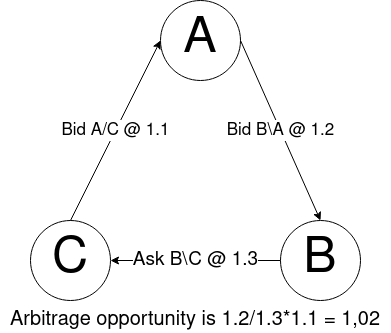
\includegraphics[width=0.4\textwidth]{assests/Flash-loans-Arbitrage-triangular}
\caption{Triangular arbitrage}
\label{fig:ArbTrig}
\end{figure}

\subsection{AMM arbitrage}
The process for detecting an arbitrage opportunity when working with AMMs, is
actually straight forward. Put simply, we just need to detect that one exchange,
has a different price than another\footnote{In our case, we have ignored fees,
but in a real system, this would of course need to be accounted for}. When we
have detected this, we need to buy at the cheaper, and sell at the more
expensive one. However, since the price at both exchanges will change as a
function of the amount of money we use, we can't just take a flash loan as big
as possible, and arbitrage with the entire amount. At some point, the price has
changed so much, that we're no longer making money, but losing it. So we need to
find the amount of money, such that when all is said and done, the two exchanges
will have the same price. Why exactly the same price? Because if the first
exchange is still lower, there still exists an arbitrage opportunity, and we
didn't fully exploit the one we found. If the second exchange is at a lower
price than the first after the transaction is done, we will have bought some of
the second asset, at a higher price, than we sold it for. While the entire
transaction might still be profitable, we didn't maximize our profits, which we
strive to do. So in order to maximize our profits, we need to find out how much
to exchange, such that the prices at the two exchanges are the same afterwards.
In the next section, we will show how to find this amount.

\subsection{Maximizing AMM arbitrage opportunities}\label{maximizing}
As explained in the previous section, the prices at the two exchanges, involved in
an arbitrage opportunity, need to be the same after the transaction, and that we
need to find the input amount (amount to be exchanged) required to maximize our
profits. In this section, we will find this amount. First, we will state the
equation that describes the desired outcome:

\begin{equation}
\overbrace{\left(\frac{x_{1b} + input}{y_{1a}}\right)}^{\text{The price at the
    first exchange, after the transaction}} = \overbrace{\left(\frac{x_{2a}}{y_{2b} + (y_{1b} - y_{1a})}\right)}^{\text{The price at the
    second exchange, after the transaction}}
\end{equation}

\begin{table}[h]
\centering
\begin{tabular}{|l|l|}
\hline
$x_{1b}$ & Amount of x, on the 1st exchange \textbf{b}efore the transaction \\
\hline
$y_{1b}$ & Amount of y, on the 1st exchange \textbf{b}efore the transaction \\
\hline
$y_{1a}$ & Amount of y, on the 1st exchange \textbf{a}fter the transaction \\
\hline
$x_{2b}$ & Amount of x, on the 2nd exchange \textbf{b}efore the transaction \\
\hline
$x_{2a}$ & Amount of x, on the 2nd exchange \textbf{a}fter the transaction \\
\hline
$y_{2b}$ & Amount of y, on the 2nd exchange \textbf{b}efore the transaction \\
\hline
\end{tabular}
\end{table}

Given that we also know that the product of the reserves, are the same before and
after the transaction, we can present the following two equations that describe
that:

\begin{equation}
\underbrace{(x_{1b} + input)}_{\text{Reserve of asset x at the 1st exchange, after transaction}} \cdot y_{1a} = x_{1b} \cdot y_{1b}
\end{equation}

\begin{equation}
x_{2a} \cdot \underbrace{(y_{2b} + (y_{1b} - y_{1a}))}_{\text{Reserve of asset y at
the 2nd exchange, after the transaction}} = x_{2b} \cdot y_{2b}
\end{equation}

We know the values of reserves before the transactions ($x_{1b}$, $y_{1b}$,
$x_{2b}$ and $y_{2b}$), we don't know the values of $input$, $y_{1a}$, and
$x_{2a}$, and we would like to find the value of $input$.

This is a simple system of 3 equations, with 3 unknowns, which can be solved
analytically. The final formula for $input$ is a quite messy
(see \ref{code:pyProf} line 10), but we can use it to find the correct amount of
$input$, in order to maximize our profits.

\subsubsection{AMM arbitrage example}
Let's say we have two exchanges with the asset pair x/y. The first exchange having
100,000 $x$, and 10,000 $y$, the second exchange having 110,000 $x$, and 10,000 $y$.
Clearly, we have an arbitrage opportunity since there will be a difference in
price. But how much should we exchange? If we enter these numbers into our
formula, we get that we should input with $2,440.44 x$. We will then convert that
into $y$, and we will end up with:

\begin{equation}
intermediary\_y = 10,000 - \frac{100,000 \cdot 10,000}{100,000 + 2,440.44} = 238.23
\end{equation}

We will then convert it back on the second exchange, and we will end up with:
\begin{equation}
resulting\_x = 110,000 - \frac{110,000 \cdot 10,000}{10,000 + 238.23} = 2559.55
\end{equation}

We now need to take into account that we started with $2,440.44 x$, and we can
calculate our profits:
\begin{equation}
profit = 2,559.55 - 2,440.44 = 119.11
\end{equation}

